\title[Resonant converters I]{Resonant converters I: SRC, PRC, LLC and CLLC}
\section{Resonant converters I}

\begin{frame}[plain]
	\titlepage
\end{frame}

%%%%%%%%%%%%%%%%%%%%%%%%%%%%%%%%%%%%%%%%%%%%%%%%%%%%%%%%%%%%%
%% Overview %%
%%%%%%%%%%%%%%%%%%%%%%%%%%%%%%%%%%%%%%%%%%%%%%%%%%%%%%%%%%%%%
\subsection{Why resonance}

\begin{frame}
	\frametitle{Overview}
	L8 took the ZVS energy from the inductor current of PWM converters. Resonant converters shape the current itself with an $LC$ tank.
	\begin{itemize}
		\item Tank fundamentals and the first-harmonic approximation (FHA)
		\item SRC, PRC and LLC: gain, ZVS and ZCS
		\item LLC design and the DC transformer (DCX) at 1\,MHz
		\item Exact analysis: state plane, operating modes, limits of FHA
		\item Bidirectional CLLC and control
	\end{itemize}
	After this lecture you can size the tank of an LLC or a DCX with FHA, check its ZVS and tell where the design must be verified in the time domain.
\end{frame}

%%%%%%%%%%%%%%%%%%%%%%%%%%%%%%%%%%%%%%%%%%%%%%%%%%%%%%%%%%%%%
%% Why resonance %%
%%%%%%%%%%%%%%%%%%%%%%%%%%%%%%%%%%%%%%%%%%%%%%%%%%%%%%%%%%%%%
\begin{frame}
	\frametitle{Why resonance at high frequency}
	\begin{columns}[T]
		\begin{column}{0.48\textwidth}
			\textbf{What the tank gives}
			\begin{itemize}
				\item ZVS of the inverter switches and ZCS of the rectifier: no $Q_\mathrm{oss}V$ loss, no reverse recovery.
				\item Parasitics become part of the tank: leakage inductance as $L_\mathrm{r}$, winding capacitance as part of $C_\mathrm{r}$ or $C_\mathrm{p}$, $C_\mathrm{oss}$ in the transition.
				\item Nearly sinusoidal currents: lower $\mathrm{d}i/\mathrm{d}t$, less EMI.
			\end{itemize}
		\end{column}
		\begin{column}{0.48\textwidth}
			\textbf{What it costs}
			\begin{itemize}
				\item Circulating current: more conduction loss.
				\item Control by frequency: a wide gain range needs a wide frequency range.
				\item High voltage or current stress of the tank elements.
				\item Tolerances of $L_\mathrm{r}$ and $C_\mathrm{r}$ shift the operating point.
			\end{itemize}
		\end{column}
	\end{columns}
	\begin{block}{Key message}
		The tank takes over the switching problem; it must be designed as carefully as the switches.
	\end{block}
\end{frame}

%%%%%%%%%%%%%%%%%%%%%%%%%%%%%%%%%%%%%%%%%%%%%%%%%%%%%%%%%%%%%
%% Structure %%
%%%%%%%%%%%%%%%%%%%%%%%%%%%%%%%%%%%%%%%%%%%%%%%%%%%%%%%%%%%%%
\begin{frame}
	\frametitle{Structure of a resonant converter}
	\begin{figure}
		\centering
		\begin{circuitikz}[scale=0.72, transform shape]
			\draw (0,0) to[V, l=$V_\mathrm{in}$] (0,4) -- (2,4) node[nigfete, anchor=D] (S1) {};
			\draw (0,0) -- (2,0) node[nigfete, anchor=S] (S2) {};
			\draw (S1.S) -- (S2.D);
			\draw (6.6,0) node[transformer core, anchor=A2] (T) {};
			\draw (2,0 |- T.A1) node[circ]{} to[C, l=$C_\mathrm{r}$] (3.8,0 |- T.A1) to[L, l=$L_\mathrm{r}$] (5.6,0 |- T.A1) node[circ]{} -- (T.A1);
			\draw (5.6,0 |- T.A1) to[L, l_=$L_\mathrm{m}$] (5.6,0) node[circ]{};
			\draw (2,0) -- (T.A2);
			\node at ($(T.A1)!0.5!(T.B1)+(0,0.5)$) {$n:1$};
			% full-bridge rectifier
			\coordinate (ra) at (9.6,0 |- T.B1);
			\draw (T.B1) -- (ra);
			\draw (9.6,0 |- T.B2) node[jump crossing] (X) {};
			\draw (T.B2) -- (X.west); \draw (X.east) -- (10.8,0 |- T.B2) coordinate (rb);
			\draw (9.6,-2.0) -- (X.south); \draw (X.north) to[D] (ra);
			\draw (ra) to[D] (9.6,4.0);
			\draw (10.8,-2.0) to[D] (rb) to[D] (10.8,4.0);
			\draw (9.6,4.0) -- (13.2,4.0); \draw (9.6,-2.0) -- (13.2,-2.0);
			\draw (12.0,4.0) to[C, l_=$C_\mathrm{o}$] (12.0,-2.0);
			\draw (13.2,4.0) to[R, l=$R_\mathrm{L}$] (13.2,-2.0);
			% blocks
			\draw[decorate, decoration={brace, amplitude=5pt, mirror}] (-0.4,-2.4) -- (2.8,-2.4) node[midway, below=6pt]{switch network};
			\draw[decorate, decoration={brace, amplitude=5pt, mirror}] (3.0,-2.4) -- (6.4,-2.4) node[midway, below=6pt]{resonant tank};
			\draw[decorate, decoration={brace, amplitude=5pt, mirror}] (6.6,-2.4) -- (13.6,-2.4) node[midway, below=6pt]{transformer, rectifier, filter};
		\end{circuitikz}
		\caption{Half-bridge LLC converter}
	\end{figure}
	\vspace{-0.3cm}
	{\small SRC: $L_\mathrm{r}$ and $C_\mathrm{r}$ in series ($L_\mathrm{m}\to\infty$). PRC: $C_\mathrm{p}$ across the transformer. LCC: both. LLC: series tank plus the magnetising inductance $L_\mathrm{m}$.}
\end{frame}

%%%%%%%%%%%%%%%%%%%%%%%%%%%%%%%%%%%%%%%%%%%%%%%%%%%%%%%%%%%%%
%% Tank fundamentals %%
%%%%%%%%%%%%%%%%%%%%%%%%%%%%%%%%%%%%%%%%%%%%%%%%%%%%%%%%%%%%%
\subsection{Tank fundamentals}

\begin{frame}
	\frametitle{Series and parallel resonance}
	\begin{columns}[T]
		\begin{column}{0.47\textwidth}
			\small
			\begin{equation*}
				\omega_\mathrm{r}=\frac{1}{\sqrt{L_\mathrm{r}C_\mathrm{r}}},\qquad Z_0=\sqrt{\frac{L_\mathrm{r}}{C_\mathrm{r}}},\qquad F=\frac{f_\mathrm{sw}}{f_\mathrm{r}}
			\end{equation*}
			Series tank with load $R$:
			\begin{equation*}
				Z=R+\mathrm{j}Z_0\left(F-\frac{1}{F}\right),\qquad Q=\frac{Z_0}{R}
			\end{equation*}
			\begin{itemize}
				\item At $f_\mathrm{r}$: $Z=R$; the voltage across $C_\mathrm{r}$ is $Q$ times that across $R$.
				\item Bandwidth $f_\mathrm{r}/Q$: the tank filters the harmonics.
				\item Parallel tank: $Q_\mathrm{p}=R/Z_0$.
			\end{itemize}
		\end{column}
		\begin{column}{0.5\textwidth}
			\begin{figure}
				\centering
				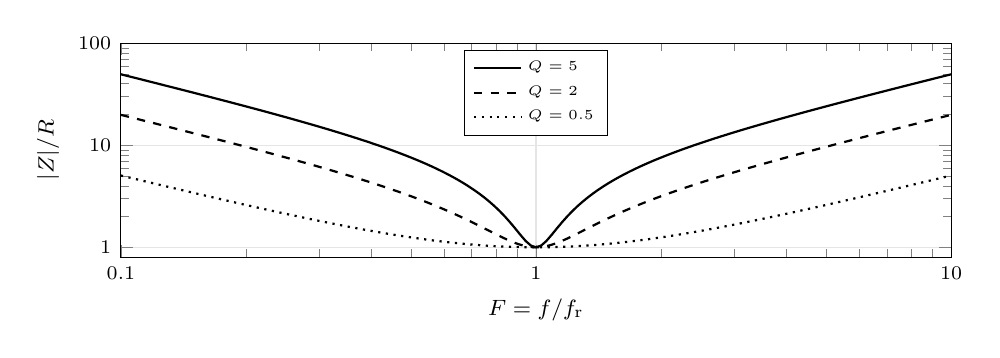
\begin{tikzpicture}
					\begin{loglogaxis}[
							width=\linewidth, height=4.3cm,
							xmin=0.1, xmax=10, ymin=0.8, ymax=100,
							xtick={0.1,1,10}, xticklabels={0.1,1,10},
							ytick={1,10,100}, yticklabels={1,10,100},
							xlabel={$F=f/f_\mathrm{r}$}, ylabel={$|Z|/R$},
							grid=major, grid style={gray!20},
							tick label style={font=\scriptsize}, label style={font=\footnotesize},
							legend style={font=\tiny, at={(0.5,0.97)}, anchor=north}, legend cell align=left,
						]
						\addplot[black, thick, domain=-1:1, samples=161] ({10^x}, {sqrt(1+25*(10^x-10^(-x))^2)});
						\addlegendentry{$Q=5$}
						\addplot[black, thick, dashed, domain=-1:1, samples=161] ({10^x}, {sqrt(1+4*(10^x-10^(-x))^2)});
						\addlegendentry{$Q=2$}
						\addplot[black, thick, dotted, domain=-1:1, samples=161] ({10^x}, {sqrt(1+0.25*(10^x-10^(-x))^2)});
						\addlegendentry{$Q=0.5$}
					\end{loglogaxis}
				\end{tikzpicture}
				\caption{Impedance of a series tank with load $R$}
			\end{figure}
		\end{column}
	\end{columns}
	\blfootnote{Sources: Erickson and Maksimovi\'c, 3rd ed., 2020, Ch.\ 22; Kazimierczuk and Czarkowski, 2011.}
\end{frame}

%%%%%%%%%%%%%%%%%%%%%%%%%%%%%%%%%%%%%%%%%%%%%%%%%%%%%%%%%%%%%
%% Task: tank at 1 MHz %%
%%%%%%%%%%%%%%%%%%%%%%%%%%%%%%%%%%%%%%%%%%%%%%%%%%%%%%%%%%%%%
% Two pages: task (page 1) and task with solution (page 2).
\begin{frame}<handout:1-2>
	\frametitle{Tank for 1\,MHz}
	\begin{block}{Task (3 minutes)}
		A series tank shall resonate at $f_\mathrm{r}=1$\,MHz with $Z_0=10\,\Omega$.
		\begin{enumerate}
			\item Calculate $L_\mathrm{r}$ and $C_\mathrm{r}$.
			\item Which voltage appears across $C_\mathrm{r}$ at resonance with 5\,A rms? Which capacitor type do you choose?
		\end{enumerate}
	\end{block}
	\onslide<2-|handout:2>{
		\begin{enumerate}
			\item $L_\mathrm{r}=Z_0/\omega_\mathrm{r}=1.59\,\mu$H, $C_\mathrm{r}=1/(\omega_\mathrm{r}Z_0)=15.9$\,nF.
			\item At $f_\mathrm{r}$ the reactance of $C_\mathrm{r}$ equals $Z_0$: 50\,V rms, 71\,V peak, in a half-bridge on top of the DC bias $V_\mathrm{in}/2$. C0G (NP0) ceramic or film capacitors: stable capacitance under bias and temperature, low loss. X7R would shift $f_\mathrm{r}$ with the voltage.
		\end{enumerate}
	}
\end{frame}

%%%%%%%%%%%%%%%%%%%%%%%%%%%%%%%%%%%%%%%%%%%%%%%%%%%%%%%%%%%%%
%% FHA %%
%%%%%%%%%%%%%%%%%%%%%%%%%%%%%%%%%%%%%%%%%%%%%%%%%%%%%%%%%%%%%
\subsection{First-harmonic approximation}

\begin{frame}
	\frametitle{The first-harmonic approximation}
	\begin{columns}[T]
		\begin{column}{0.5\textwidth}
			\begin{figure}
				\centering
				\begin{circuitikz}[scale=0.75, transform shape]
					\draw (0,0) to[sV, l=$v_\mathrm{s1}$] (0,2.5) to[C, l=$C_\mathrm{r}$] (2,2.5) to[L, l=$L_\mathrm{r}$] (4,2.5) -- (5.5,2.5);
					\draw (4,2.5) node[circ]{} to[L, l_=$L_\mathrm{m}$] (4,0) node[circ]{};
					\draw (5.5,2.5) to[R, l_=$R_\mathrm{e}$, v^>=$v_\mathrm{o1}$] (5.5,0) -- (0,0);
				\end{circuitikz}
				\caption{FHA equivalent circuit of the LLC}
			\end{figure}
		\end{column}
		\begin{column}{0.47\textwidth}
			\small
			Assumptions:
			\begin{enumerate}
				\item Only the fundamental transfers power; the tank filters the harmonics.
				\item The rectifier with its filter and load behaves like a resistance $R_\mathrm{e}$.
				\item Losses and the dead time are neglected.
			\end{enumerate}
			The converter becomes a linear AC circuit: gain, currents and input phase follow from phasors.
			\vspace{0.2cm}

			FHA is accurate near $f_\mathrm{r}$, where the tank filters well. Far from resonance, and below it in particular, it must be checked in the time domain.
		\end{column}
	\end{columns}
	\blfootnote{Source: R.\,L. Steigerwald, IEEE Trans.\ Power Electron., vol.\ 3, no.\ 2, 1988.}
\end{frame}

%%%%%%%%%%%%%%%%%%%%%%%%%%%%%%%%%%%%%%%%%%%%%%%%%%%%%%%%%%%%%
%% Inverter and rectifier in FHA %%
%%%%%%%%%%%%%%%%%%%%%%%%%%%%%%%%%%%%%%%%%%%%%%%%%%%%%%%%%%%%%
\begin{frame}
	\frametitle{Inverter and rectifier in FHA}
	\begin{columns}[T]
		\begin{column}{0.48\textwidth}
			\small
			\textbf{Inverter}: a square wave of amplitude $V$ has the fundamental $4V/\pi$:
			\begin{itemize}
				\item half-bridge ($V=V_\mathrm{in}/2$): $\hat{v}_\mathrm{s1}=2V_\mathrm{in}/\pi$
				\item full bridge ($V=V_\mathrm{in}$): $\hat{v}_\mathrm{s1}=4V_\mathrm{in}/\pi$
			\end{itemize}
			\textbf{Rectifier with capacitive filter}: the winding sees $\pm nV_\mathrm{o}$ in phase with the sinusoidal current $\hat{\imath}_\mathrm{p}$:
			\begin{equation*}
				\hat{v}_\mathrm{o1}=\frac{4nV_\mathrm{o}}{\pi},\qquad I_\mathrm{o}=\frac{2n\hat{\imath}_\mathrm{p}}{\pi}
			\end{equation*}
			\begin{equation*}
				R_\mathrm{e}=\frac{\hat{v}_\mathrm{o1}}{\hat{\imath}_\mathrm{p}}=\frac{8n^2}{\pi^2}R_\mathrm{L}
			\end{equation*}
		\end{column}
		\begin{column}{0.48\textwidth}
			\small
			\textbf{Rectifier with inductive filter} (PRC): the rectifier draws a square-wave current, the voltage is sinusoidal:
			\begin{equation*}
				R_\mathrm{e}=\frac{\pi^2n^2}{8}R_\mathrm{L}
			\end{equation*}
			\textbf{Gain}: with $M=nV_\mathrm{o}/V$ the ratio of the DC voltages equals the ratio of the fundamentals:
			\begin{equation*}
				M=\left|\frac{\underline{v}_\mathrm{o1}}{\underline{v}_\mathrm{s1}}\right|
			\end{equation*}
			Everything else is AC circuit analysis.
		\end{column}
	\end{columns}
	\blfootnote{Sources: Steigerwald, 1988; Erickson and Maksimovi\'c, 2020, Ch.\ 22.}
\end{frame}

%%%%%%%%%%%%%%%%%%%%%%%%%%%%%%%%%%%%%%%%%%%%%%%%%%%%%%%%%%%%%
%% Task: Re %%
%%%%%%%%%%%%%%%%%%%%%%%%%%%%%%%%%%%%%%%%%%%%%%%%%%%%%%%%%%%%%
% Two pages: task (page 1) and task with solution (page 2).
\begin{frame}<handout:1-2>
	\frametitle{Equivalent load resistance}
	\begin{block}{Task (3 minutes)}
		A full-bridge rectifier with capacitive output filter supplies 12\,V and 20\,A through a transformer with $n=4$.
		\begin{enumerate}
			\item Calculate $R_\mathrm{e}$ seen by the tank.
			\item With $Z_0=10\,\Omega$ (previous task): which $Q$ results, and how large is the third-harmonic current relative to the fundamental at $f_\mathrm{r}$?
		\end{enumerate}
	\end{block}
	\onslide<2-|handout:2>{
		\begin{enumerate}
			\item $R_\mathrm{L}=0.6\,\Omega$, $R_\mathrm{e}=8\cdot16\cdot0.6\,\Omega/\pi^2=7.8\,\Omega$ (with an inductive filter 11.8\,$\Omega$).
			\item $Q=Z_0/R_\mathrm{e}=1.29$. The third harmonic has 1/3 of the voltage and sees $|Z|=R_\mathrm{e}\sqrt{1+Q^2(3-1/3)^2}=3.6R_\mathrm{e}$: 9\,\% of the fundamental current. The fifth: 3\,\%. FHA is reasonable here.
		\end{enumerate}
	}
\end{frame}

%%%%%%%%%%%%%%%%%%%%%%%%%%%%%%%%%%%%%%%%%%%%%%%%%%%%%%%%%%%%%
%% SRC and PRC %%
%%%%%%%%%%%%%%%%%%%%%%%%%%%%%%%%%%%%%%%%%%%%%%%%%%%%%%%%%%%%%
\begin{frame}
	\frametitle{Series and parallel resonant converter}
	\begin{columns}[T]
		\begin{column}{0.49\textwidth}
			\begin{figure}
				\centering
				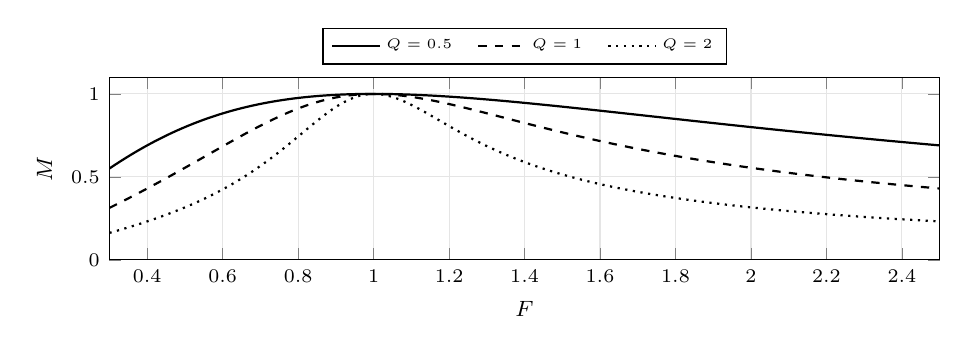
\begin{tikzpicture}
					\begin{axis}[
							width=\linewidth, height=3.9cm,
							xmin=0.3, xmax=2.5, ymin=0, ymax=1.1,
							xlabel={$F$}, ylabel={$M$},
							grid=major, grid style={gray!20},
							tick label style={font=\scriptsize}, label style={font=\footnotesize},
							legend style={font=\tiny, at={(0.5,1.07)}, anchor=south, legend columns=3, /tikz/every even column/.append style={column sep=0.25cm}}, legend cell align=left,
						]
						\addplot[black, thick, domain=0.3:2.5, samples=150] {1/sqrt(1+0.25*(x-1/x)^2)};
						\addlegendentry{$Q=0.5$}
						\addplot[black, thick, dashed, domain=0.3:2.5, samples=150] {1/sqrt(1+(x-1/x)^2)};
						\addlegendentry{$Q=1$}
						\addplot[black, thick, dotted, domain=0.3:2.5, samples=150] {1/sqrt(1+4*(x-1/x)^2)};
						\addlegendentry{$Q=2$}
					\end{axis}
				\end{tikzpicture}
				\caption{SRC: $M=1\big/\sqrt{1+Q^2(F-1/F)^2}$}
			\end{figure}
		\end{column}
		\begin{column}{0.49\textwidth}
			\begin{figure}
				\centering
				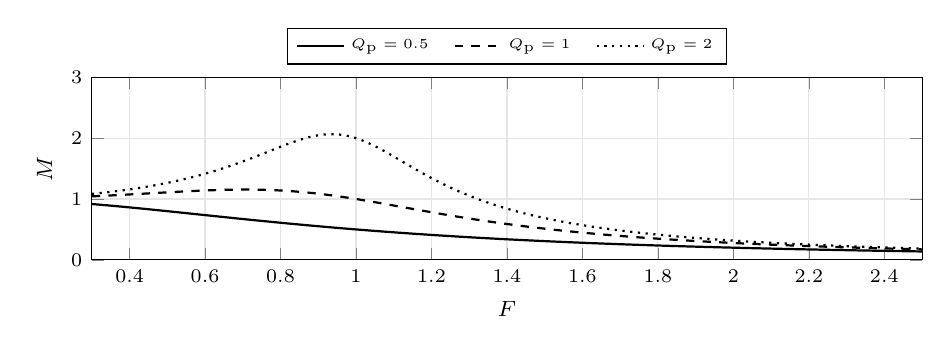
\begin{tikzpicture}
					\begin{axis}[
							width=\linewidth, height=3.9cm,
							xmin=0.3, xmax=2.5, ymin=0, ymax=3,
							xlabel={$F$}, ylabel={$M$},
							grid=major, grid style={gray!20},
							tick label style={font=\scriptsize}, label style={font=\footnotesize},
							legend style={font=\tiny, at={(0.5,1.07)}, anchor=south, legend columns=3, /tikz/every even column/.append style={column sep=0.25cm}}, legend cell align=left,
						]
						\addplot[black, thick, domain=0.3:2.5, samples=200] {1/sqrt((1-x^2)^2+(x/0.5)^2)};
						\addlegendentry{$Q_\mathrm{p}=0.5$}
						\addplot[black, thick, dashed, domain=0.3:2.5, samples=200] {1/sqrt((1-x^2)^2+(x/1)^2)};
						\addlegendentry{$Q_\mathrm{p}=1$}
						\addplot[black, thick, dotted, domain=0.3:2.5, samples=200] {1/sqrt((1-x^2)^2+(x/2)^2)};
						\addlegendentry{$Q_\mathrm{p}=2$}
					\end{axis}
				\end{tikzpicture}
				\caption{PRC: $M=1\big/\sqrt{(1-F^2)^2+(F/Q_\mathrm{p})^2}$}
			\end{figure}
		\end{column}
	\end{columns}
	\vspace{-0.2cm}
	{\small SRC: $M\leq1$; at light load ($Q\to0$) $M\to1$ at every frequency, so it cannot regulate without load, and its current vanishes. PRC: boosts and regulates without load, but the current in $C_\mathrm{p}$ does not fall with the load.}
	\blfootnote{Source: Steigerwald, 1988.}
\end{frame}

%%%%%%%%%%%%%%%%%%%%%%%%%%%%%%%%%%%%%%%%%%%%%%%%%%%%%%%%%%%%%
%% Above or below resonance %%
%%%%%%%%%%%%%%%%%%%%%%%%%%%%%%%%%%%%%%%%%%%%%%%%%%%%%%%%%%%%%
\begin{frame}
	\frametitle{Above or below resonance}
	\begin{columns}[T]
		\begin{column}{0.48\textwidth}
			\begin{figure}
				\centering
				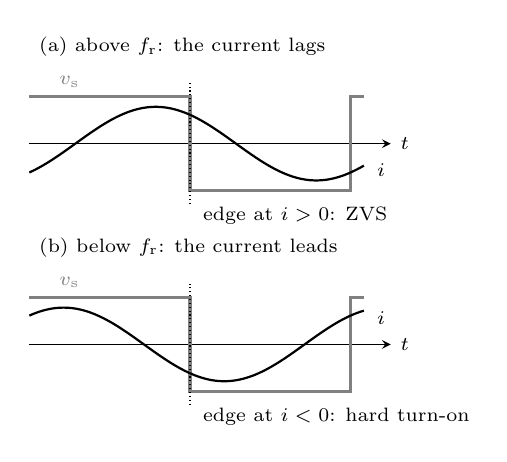
\begin{tikzpicture}[scale=0.85, >=stealth, font=\scriptsize]
					% (a) above resonance: current lags
					\node[anchor=west] at (0,3.85) {(a) above $f_\mathrm{r}$: the current lags};
					\draw[->] (0,2.4) -- (5.4,2.4) node[right]{$t$};
					\draw[gray, line width=1.2pt] (0,3.1) -- (2.4,3.1) -- (2.4,1.7) -- (4.8,1.7) -- (4.8,3.1) -- (5.0,3.1);
					\draw[thick, domain=0:5.0, samples=100, smooth] plot (\x, {2.4+0.55*sin(deg(pi*\x/2.4-0.9))});
					\node[gray, anchor=south] at (0.6,3.1) {$v_\mathrm{s}$};
					\node[anchor=west] at (5.05,2.0) {$i$};
					\draw[densely dotted] (2.4,1.5) -- (2.4,3.3);
					\node[anchor=north west] at (2.45,1.6) {edge at $i>0$: ZVS};
					% (b) below resonance: current leads
					\node[anchor=west] at (0,0.85) {(b) below $f_\mathrm{r}$: the current leads};
					\draw[->] (0,-0.6) -- (5.4,-0.6) node[right]{$t$};
					\draw[gray, line width=1.2pt] (0,0.1) -- (2.4,0.1) -- (2.4,-1.3) -- (4.8,-1.3) -- (4.8,0.1) -- (5.0,0.1);
					\draw[thick, domain=0:5.0, samples=100, smooth] plot (\x, {-0.6+0.55*sin(deg(pi*\x/2.4+0.9))});
					\node[gray, anchor=south] at (0.6,0.1) {$v_\mathrm{s}$};
					\node[anchor=west] at (5.05,-0.2) {$i$};
					\draw[densely dotted] (2.4,-1.5) -- (2.4,0.3);
					\node[anchor=north west] at (2.45,-1.4) {edge at $i<0$: hard turn-on};
				\end{tikzpicture}
				\caption{Grey: bridge voltage $v_\mathrm{s}$; black: tank current $i$; dotted: a bridge edge}
			\end{figure}
		\end{column}
		\begin{column}{0.49\textwidth}
			\small
			\textbf{Inductive input (above $f_\mathrm{r}$ in the SRC)}: the current lags. When a switch turns off, the current flows towards the other switch and discharges it: ZVS turn-on. Turn-off is hard but cushioned by $C_\mathrm{oss}$.
			\vspace{0.2cm}

			\textbf{Capacitive input}: the current leads and has already reversed. The switches turn off at zero current (ZCS), but turn on hard: $Q_\mathrm{oss}V$ loss and reverse recovery of the opposite body diode.
			\vspace{0.2cm}

			MOSFETs and GaN: always inductive. Capacitive operation suits thyristors (natural commutation) and partly IGBTs (tail current).
		\end{column}
	\end{columns}
\end{frame}

%%%%%%%%%%%%%%%%%%%%%%%%%%%%%%%%%%%%%%%%%%%%%%%%%%%%%%%%%%%%%
%% LLC %%
%%%%%%%%%%%%%%%%%%%%%%%%%%%%%%%%%%%%%%%%%%%%%%%%%%%%%%%%%%%%%
\subsection{LLC and DC transformer}

\begin{frame}
	\frametitle{The LLC converter}
	\begin{columns}[T]
		\begin{column}{0.5\textwidth}
			\begin{figure}
				\centering
				\begin{tikzpicture}
					\begin{axis}[
							width=\linewidth, height=5.0cm,
							xmin=0.3, xmax=2.0, ymin=0, ymax=3,
							xlabel={$F=f_\mathrm{sw}/f_\mathrm{r}$}, ylabel={$M$},
							grid=major, grid style={gray!20},
							tick label style={font=\scriptsize}, label style={font=\footnotesize},
							legend style={font=\tiny, at={(0.97,0.97)}, anchor=north east}, legend cell align=left,
						]
						\addplot[black, thick, domain=0.3:2, samples=300] {abs(5*x^2/sqrt((6*x^2-1)^2+((x^2-1)*x*0.2*5)^2))};
						\addlegendentry{$Q=0.2$}
						\addplot[black, thick, dashed, domain=0.3:2, samples=300] {abs(5*x^2/sqrt((6*x^2-1)^2+((x^2-1)*x*0.5*5)^2))};
						\addlegendentry{$Q=0.5$}
						\addplot[black, thick, dotted, domain=0.3:2, samples=300] {abs(5*x^2/sqrt((6*x^2-1)^2+((x^2-1)*x*1*5)^2))};
						\addlegendentry{$Q=1$}
						\addplot[black, thick, dashdotted, domain=0.3:2, samples=300] {abs(5*x^2/sqrt((6*x^2-1)^2+((x^2-1)*x*2*5)^2))};
						\addlegendentry{$Q=2$}
						\addplot[gray, thin] table[x=F, y=M] {fig/lec09/llc_boundary.dat};
						\node[font=\tiny, anchor=west, gray] at (axis cs:0.5,2.6) {ZVS limit};
					\end{axis}
				\end{tikzpicture}
				\caption{FHA gain of the LLC, $L_\mathrm{n}=5$; left of the grey line the input is capacitive}
			\end{figure}
		\end{column}
		\begin{column}{0.47\textwidth}
			\small
			With $L_\mathrm{n}=L_\mathrm{m}/L_\mathrm{r}$, $F=f_\mathrm{sw}/f_\mathrm{r}$, $Q=Z_0/R_\mathrm{e}$:
			\begin{equation*}
				M=\left|\frac{L_\mathrm{n}F^2}{\left[(L_\mathrm{n}+1)F^2-1\right]+\mathrm{j}\left(F^2-1\right)FQL_\mathrm{n}}\right|
			\end{equation*}
			\begin{itemize}
				\item $M=1$ at $F=1$ for every load.
				\item Below $f_\mathrm{r}$ the gain rises above 1; the peak lies near the ZVS limit.
				\item The second resonance $f_0=f_\mathrm{r}/\sqrt{1+L_\mathrm{n}}$ bounds the useful range.
				\item $L_\mathrm{m}$ carries a current at every load: ZVS also without load.
			\end{itemize}
		\end{column}
	\end{columns}
	\blfootnote{Sources: Steigerwald, 1988; B. Lu et al., IEEE APEC 2006.}
\end{frame}

%%%%%%%%%%%%%%%%%%%%%%%%%%%%%%%%%%%%%%%%%%%%%%%%%%%%%%%%%%%%%
%% Poll: ZCS of the rectifier %%
%%%%%%%%%%%%%%%%%%%%%%%%%%%%%%%%%%%%%%%%%%%%%%%%%%%%%%%%%%%%%
% Two pages: question (page 1) and answer (page 2).
\begin{frame}<handout:1-2>
	\frametitle{Where does the rectifier switch softly?}
	\begin{columns}[T]
		\begin{column}{0.48\textwidth}
			\small
			Poll: in which range does the LLC rectifier turn off at zero current (ZCS)?
			\begin{enumerate}[A]
				\item above $f_\mathrm{r}$
				\item between the ZVS limit and $f_\mathrm{r}$
				\item below the ZVS limit
				\item at every frequency
			\end{enumerate}
		\end{column}
		\begin{column}{0.48\textwidth}
			\onslide<2-|handout:2>{
				\begin{block}{Answer: B (and at $f_\mathrm{r}$)}
					Below $f_\mathrm{r}$ the series resonance completes its half cycle before the bridge switches; the rectifier current returns to zero and $L_\mathrm{m}$ takes over the tank current: ZCS of the rectifier, ZVS of the bridge. Above $f_\mathrm{r}$ the bridge interrupts the half sine and commutates the rectifier current. Below the ZVS limit the bridge loses ZVS.
				\end{block}
			}
		\end{column}
	\end{columns}
\end{frame}

%%%%%%%%%%%%%%%%%%%%%%%%%%%%%%%%%%%%%%%%%%%%%%%%%%%%%%%%%%%%%
%% LLC design %%
%%%%%%%%%%%%%%%%%%%%%%%%%%%%%%%%%%%%%%%%%%%%%%%%%%%%%%%%%%%%%
\begin{frame}
	\frametitle{LLC design flow}
	\begin{enumerate}
		\item Gain range from the input- and output-voltage ranges, e.g.\ $M=nV_\mathrm{o}/V$ from 0.9 to 1.3.
		\item Choose $L_\mathrm{n}$ (typically 3 to 10) and the full-load $Q$ so that the peak gain lies above $M_\mathrm{max}$ with margin. A small $L_\mathrm{n}$ gives more gain, but a larger magnetising current.
		\item $f_\mathrm{r}$ near the target frequency; $R_\mathrm{e}$ from the full load; $Z_0=QR_\mathrm{e}$, $L_\mathrm{r}=Z_0/\omega_\mathrm{r}$, $C_\mathrm{r}=1/(\omega_\mathrm{r}Z_0)$, $L_\mathrm{m}=L_\mathrm{n}L_\mathrm{r}$.
		\item ZVS: the magnetising current must move the charge within the dead time (next slide). If it cannot, reduce $L_\mathrm{m}$ and repeat.
		\item Check the corners of the operating range in the time domain; FHA is least accurate below resonance.
	\end{enumerate}
	\begin{block}{Key message}
		$L_\mathrm{m}$ is a compromise: small enough for ZVS, large enough to keep the circulating current and the turn-off current low.
	\end{block}
	\blfootnote{Source: B. Lu, W. Liu, Y. Liang, F.\,C. Lee, J.\,D. van Wyk, IEEE APEC 2006, pp.\ 533--538.}
\end{frame}

%%%%%%%%%%%%%%%%%%%%%%%%%%%%%%%%%%%%%%%%%%%%%%%%%%%%%%%%%%%%%
%% ZVS of the LLC %%
%%%%%%%%%%%%%%%%%%%%%%%%%%%%%%%%%%%%%%%%%%%%%%%%%%%%%%%%%%%%%
\begin{frame}
	\frametitle{ZVS of the LLC}
	\begin{columns}[T]
		\begin{column}{0.5\textwidth}
			\small
			At $f_\mathrm{r}$ the magnetising inductance sees $\pm nV_\mathrm{o}$; its triangular current peaks at the switching instant:
			\begin{equation*}
				I_\mathrm{m,pk}=\frac{nV_\mathrm{o}}{4f_\mathrm{sw}L_\mathrm{m}}
			\end{equation*}
			The inductor ends at the midpoint of the bus ($V_x=V/2$, L8): no energy is needed, only the charge within the dead time:
			\begin{align*}
				I_\mathrm{m,pk}               & \geq\frac{2Q_\mathrm{oss}+Q_\mathrm{TR}}{t_\mathrm{d}}                                    \\
				\Rightarrow\quad L_\mathrm{m} & \leq\frac{nV_\mathrm{o}\,t_\mathrm{d}}{4f_\mathrm{sw}(2Q_\mathrm{oss}+Q_\mathrm{TR})}
			\end{align*}
		\end{column}
		\begin{column}{0.47\textwidth}
			\small
			\begin{itemize}
				\item $Q_\mathrm{TR}$: charge of the transformer and winding capacitance, often comparable to $Q_\mathrm{oss}$ in planar transformers (L7).
				\item The bridge turns off with $I_\mathrm{m,pk}$: a larger $I_\mathrm{m,pk}$ secures ZVS but raises turn-off and conduction loss.
				\item Lu et al.\ choose $L_\mathrm{m}$ so that $I_\mathrm{m,pk}$ just meets the ZVS requirement.
				\item Most critical: the highest switching frequency at light load, where $nV_\mathrm{o}/(4f_\mathrm{sw}L_\mathrm{m})$ is smallest and the load current adds little.
			\end{itemize}
		\end{column}
	\end{columns}
	\blfootnote{Sources: Lu et al., APEC 2006; Lecture 8.}
\end{frame}

%%%%%%%%%%%%%%%%%%%%%%%%%%%%%%%%%%%%%%%%%%%%%%%%%%%%%%%%%%%%%
%% DCX %%
%%%%%%%%%%%%%%%%%%%%%%%%%%%%%%%%%%%%%%%%%%%%%%%%%%%%%%%%%%%%%
\begin{frame}
	\frametitle{The DC transformer}
	\small
	An LLC operated open-loop at $f_\mathrm{r}$: $M=1$ independent of the load, so $V_\mathrm{o}=V_\mathrm{in}/n$ (full bridge), like an ideal transformer, with ZVS, ZCS and nearly sinusoidal currents at one fixed frequency. Regulation is left to another stage: 48\,V bus $\rightarrow$ DCX $\rightarrow$ 12\,V $\rightarrow$ point-of-load regulators.
	\begin{table}
		\centering
		\scriptsize
		\begin{tabular}{|l|l|l|l|}
			\hline
			$R_\mathrm{L}$, $R_\mathrm{e}$                         & 0.576\,$\Omega$, 7.47\,$\Omega$                       & $L_\mathrm{r}$ (leakage, Tutorial 7) & 37\,nH                    \\
			ZVS ($Q_\mathrm{oss}=10$\,nC, $t_\mathrm{d}=10$\,ns) & $I_\mathrm{m,pk}\geq2$\,A: $L_\mathrm{m}\leq6\,\mu$H & $C_\mathrm{r}$ (C0G)                 & 685\,nF                   \\
			$L_\mathrm{m}$ (gap 0.14\,mm)                         & 5\,$\mu$H, $I_\mathrm{m,pk}=2.4$\,A                  & $Z_0$, $Q$, $L_\mathrm{n}$           & 0.23\,$\Omega$, 0.03, 135  \\
			secondary peak current                                & 32.7\,A (half sines)                                 & primary rms current                  & 5.95\,A                   \\
			\hline
		\end{tabular}
		\caption{B2: 48\,V to 12\,V, 250\,W, 1\,MHz, $n=4$, full bridge}
	\end{table}
	With $Q=0.03$ and $L_\mathrm{n}=135$ the gain changes by only 0.2\,\% for $\pm10$\,\% frequency deviation: the DCX tolerates the scatter of $f_\mathrm{r}$, but it cannot regulate. $C_\mathrm{r}$ carries only 1.9\,V peak ripple.
	\blfootnote{Core of Tutorial 6, Task 3 ($A_\mathrm{e}=40$\,mm$^2$, $l_\mathrm{e}=25$\,mm, $\mu_\mathrm{r}\approx1000$); transistors of Tutorial 8.}
\end{frame}

%%%%%%%%%%%%%%%%%%%%%%%%%%%%%%%%%%%%%%%%%%%%%%%%%%%%%%%%%%%%%
%% SR timing %%
%%%%%%%%%%%%%%%%%%%%%%%%%%%%%%%%%%%%%%%%%%%%%%%%%%%%%%%%%%%%%
\begin{frame}
	\frametitle{Synchronous rectifiers at 1\,MHz}
	\begin{columns}[T]
		\begin{column}{0.48\textwidth}
			\begin{figure}
				\centering
				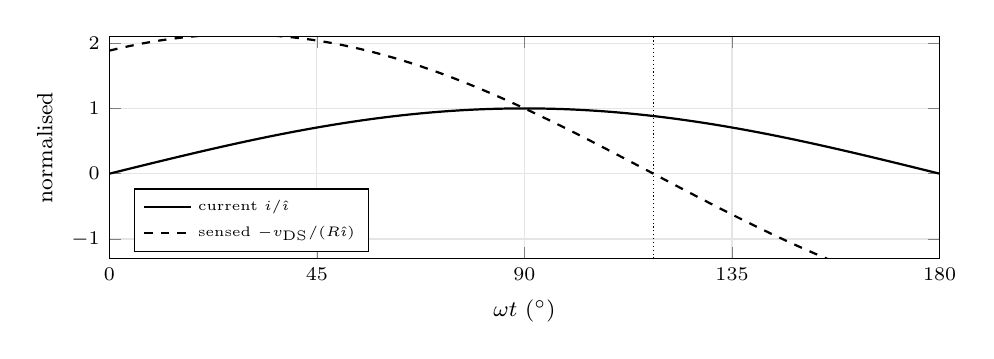
\begin{tikzpicture}
					\begin{axis}[
							width=\linewidth, height=4.4cm,
							xmin=0, xmax=180, ymin=-1.3, ymax=2.1,
							xtick={0,45,90,135,180},
							xlabel={$\omega t$ ($^\circ$)}, ylabel={normalised},
							grid=major, grid style={gray!20},
							tick label style={font=\scriptsize}, label style={font=\footnotesize},
							legend style={font=\tiny, at={(0.03,0.03)}, anchor=south west}, legend cell align=left,
						]
						\addplot[black, thick, domain=0:180, samples=100] {sin(x)};
						\addlegendentry{current $i/\hat{\imath}$}
						\addplot[black, thick, dashed, domain=0:180, samples=100] {sin(x)+1.885*cos(x)};
						\addlegendentry{sensed $-v_\mathrm{DS}/(R\hat{\imath})$}
						\addplot[black, densely dotted] coordinates {(118,-1.3) (118,2.1)};
					\end{axis}
				\end{tikzpicture}
				\caption{Rectifier current and sensed voltage; 1\,MHz, $R_\mathrm{DS(on)}=1$\,m$\Omega$, 0.3\,nH}
			\end{figure}
		\end{column}
		\begin{column}{0.49\textwidth}
			\footnotesize
			A controller that turns the SR off when $v_\mathrm{DS}$ crosses zero sees $R_\mathrm{DS(on)}i+L_\mathrm{pkg}\,\mathrm{d}i/\mathrm{d}t$ (package inductance in the sense path), not only $R_\mathrm{DS(on)}i$. The sensed zero comes early by
			\begin{equation*}
				\Delta\theta=\arctan\frac{\omega L_\mathrm{pkg}}{R_\mathrm{DS(on)}}
			\end{equation*}
			\begin{itemize}
				\item 0.3\,nH, 1\,m$\Omega$: $62^\circ$ (172\,ns) early; the GaN SR conducts in reverse at about 2\,V for the rest: 5.5\,W per device in B2, each 2\,\% of 250\,W.
				\item At 100\,kHz the same layout gives $11^\circ$.
				\item Remedies: drive the SRs from the primary timing (in a DCX at $f_\mathrm{r}$ the secondary current is in phase), compensate $L\,\mathrm{d}i/\mathrm{d}t$ in the sensing, adaptive digital timing.
			\end{itemize}
		\end{column}
	\end{columns}
\end{frame}

%%%%%%%%%%%%%%%%%%%%%%%%%%%%%%%%%%%%%%%%%%%%%%%%%%%%%%%%%%%%%
%% Transformer and tank components %%
%%%%%%%%%%%%%%%%%%%%%%%%%%%%%%%%%%%%%%%%%%%%%%%%%%%%%%%%%%%%%
\begin{frame}
	\frametitle{Transformer and tank components}
	\begin{itemize}
		\item $L_\mathrm{r}$ from the leakage of the transformer: repeatable in a planar stack (L7); a magnetic shunt or a small air-core inductor adds more.
		\item Matrix transformer: several elementary transformers with one secondary turn each, primaries in series, secondaries in parallel. 390\,V to 12\,V, 1\,kW, 1\,MHz, 95.4\,\% (Huang, Ji, Lee, 2014).
		\item Split-phase fractional-turn transformer: 380\,V to 12\,V, 1\,kW, 1\,MHz, 97.7\,\% peak (Ranjram and Perreault, 2022).
		\item $C_\mathrm{r}$: C0G ceramic or film. X7R loses a large part of its capacitance with DC bias and temperature, and $f_\mathrm{r}\propto1/\sqrt{L_\mathrm{r}C_\mathrm{r}}$ moves with it.
		\item Tolerances: $\pm10$\,\% on $L_\mathrm{r}$ and $\pm5$\,\% on $C_\mathrm{r}$ move $f_\mathrm{r}$ by up to $\pm8$\,\%. A DCX is tuned to the measured $f_\mathrm{r}$; an LLC keeps gain margin.
	\end{itemize}
	\blfootnote{Sources: D. Huang, S. Ji, F.\,C. Lee, IEEE TPEL, vol.\ 29, no.\ 8, 2014; M.\,K. Ranjram, D.\,J. Perreault, IEEE TPEL, vol.\ 37, no.\ 2, 2022.}
\end{frame}

%%%%%%%%%%%%%%%%%%%%%%%%%%%%%%%%%%%%%%%%%%%%%%%%%%%%%%%%%%%%%
%% Exact analysis %%
%%%%%%%%%%%%%%%%%%%%%%%%%%%%%%%%%%%%%%%%%%%%%%%%%%%%%%%%%%%%%
\subsection{Exact analysis}

\begin{frame}
	\frametitle{Exact analysis in the time domain}
	\begin{columns}[T]
		\begin{column}{0.5\textwidth}
			\small
			Between two events (bridge edge, rectifier on or off) the tank is linear and sees a constant voltage $V_\mathrm{s}$:
			\begin{align*}
				v_C(t)-V_\mathrm{s} & =(v_{C0}-V_\mathrm{s})\cos\omega_\mathrm{r}t+Z_0i_0\sin\omega_\mathrm{r}t \\
				Z_0i(t)            & =Z_0i_0\cos\omega_\mathrm{r}t-(v_{C0}-V_\mathrm{s})\sin\omega_\mathrm{r}t
			\end{align*}
			In the normalised state plane ($m_C=v_C/V$, $j=Z_0i/V$) each interval is an arc of a circle around $(V_\mathrm{s}/V,\,0)$.
		\end{column}
		\begin{column}{0.47\textwidth}
			\small
			\begin{itemize}
				\item Steady state: the trajectory closes after one period, by symmetry after half a period with reversed sign.
				\item Solved graphically (state plane), analytically mode by mode, or numerically (shooting method, L8).
				\item Gives peak currents and capacitor voltages directly: the radius of the arcs.
				\item In the LLC the rectifier can be off: then $L_\mathrm{r}+L_\mathrm{m}$ resonate with $C_\mathrm{r}$ at $f_0$.
			\end{itemize}
		\end{column}
	\end{columns}
	\blfootnote{Source: Erickson and Maksimovi\'c, 2020, Ch.\ 22 (exact characteristics of the SRC and PRC).}
\end{frame}

%%%%%%%%%%%%%%%%%%%%%%%%%%%%%%%%%%%%%%%%%%%%%%%%%%%%%%%%%%%%%
%% State plane %%
%%%%%%%%%%%%%%%%%%%%%%%%%%%%%%%%%%%%%%%%%%%%%%%%%%%%%%%%%%%%%
\begin{frame}
	\frametitle{State plane of the SRC}
	\begin{columns}[T]
		\begin{column}{0.5\textwidth}
			\begin{figure}
				\centering
				\begin{tikzpicture}
					\begin{axis}[
							width=\linewidth, height=5.2cm,
							axis equal image,
							xmin=-2.4, xmax=2.4, ymin=-1.3, ymax=1.3,
							xlabel={$m_C=v_C/V_\mathrm{in}$}, ylabel={$j=Z_0i/V_\mathrm{in}$},
							grid=major, grid style={gray!20},
							tick label style={font=\scriptsize}, label style={font=\footnotesize},
						]
						\addplot[black, thick] table[x=mc, y=j] {fig/lec09/src_plane.dat};
						\addplot[only marks, mark=+, mark size=2pt] coordinates {(0.106,0) (1.894,0) (-0.106,0) (-1.894,0)};
						\node[font=\tiny, anchor=south] at (axis cs:1.894,0.05) {$1+M$};
						\node[font=\tiny, anchor=north] at (axis cs:0.106,-0.05) {$1-M$};
					\end{axis}
				\end{tikzpicture}
				\caption{Exact steady state, $F=1.2$, $Q=1$}
			\end{figure}
		\end{column}
		\begin{column}{0.47\textwidth}
			\small
			Full-bridge SRC, bridge voltage $\pm V_\mathrm{in}$, rectifier voltage $\pm nV_\mathrm{o}=\pm MV_\mathrm{in}$:
			\begin{itemize}
				\item With $v_\mathrm{s}=+V_\mathrm{in}$ the tank sees $V_\mathrm{s}=V_\mathrm{in}\pm MV_\mathrm{in}$, depending on the sign of $i$: an arc around $m_C=1+M$ while $i<0$, around $1-M$ while $i>0$.
				\item The second half period is the mirror image around the origin.
				\item Above resonance the current is still negative after the bridge edge: ZVS.
				\item Exact gain here 0.894; FHA gives 0.939 (5\,\% high).
			\end{itemize}
		\end{column}
	\end{columns}
	\blfootnote{Simulation: time-domain steady state with ideal switches and rectifier (\texttt{lecture/sim/llc\_timedomain.py}).}
\end{frame}

%%%%%%%%%%%%%%%%%%%%%%%%%%%%%%%%%%%%%%%%%%%%%%%%%%%%%%%%%%%%%
%% LLC operating modes %%
%%%%%%%%%%%%%%%%%%%%%%%%%%%%%%%%%%%%%%%%%%%%%%%%%%%%%%%%%%%%%
\begin{frame}
	\frametitle{Operating modes of the LLC}
	\begin{figure}
		\centering
		\begin{tikzpicture}
			\begin{groupplot}[
					group style={group size=3 by 1, horizontal sep=0.9cm, yticklabels at=edge left},
					width=5.2cm, height=4.0cm,
					xmin=0, xmax=6.2832, ymin=-1.05, ymax=1.05,
					xtick={0,3.1416,6.2832}, xticklabels={0,$\pi$,$2\pi$},
					xlabel={$\omega_\mathrm{sw}t$},
					grid=major, grid style={gray!20},
					tick label style={font=\scriptsize}, label style={font=\footnotesize}, title style={font=\footnotesize},
				]
				\nextgroupplot[title={$F=0.8$: rectifier off before the edge}, ylabel={$Z_0i/V_\mathrm{in}$}]
				\addplot[black, thick] table[x=th, y=ir08] {fig/lec09/llc_modes.dat};
				\addplot[black, dashed] table[x=th, y=im08] {fig/lec09/llc_modes.dat};
				\nextgroupplot[title={$F=1$: half sines}]
				\addplot[black, thick] table[x=th, y=ir10] {fig/lec09/llc_modes.dat};
				\addplot[black, dashed] table[x=th, y=im10] {fig/lec09/llc_modes.dat};
				\nextgroupplot[title={$F=1.3$: half sine interrupted}]
				\addplot[black, thick] table[x=th, y=ir13] {fig/lec09/llc_modes.dat};
				\addplot[black, dashed] table[x=th, y=im13] {fig/lec09/llc_modes.dat};
			\end{groupplot}
		\end{tikzpicture}
		\caption{Tank current $i_\mathrm{r}$ (solid) and magnetising current $i_\mathrm{m}$ (dashed), exact steady state, $L_\mathrm{n}=5$, $Q=0.5$; the rectifier current is $i_\mathrm{r}-i_\mathrm{m}$}
	\end{figure}
	\vspace{-0.2cm}
	{\small Below $f_\mathrm{r}$: $i_\mathrm{r}$ meets $i_\mathrm{m}$ before the bridge edge, the rectifier current ends at zero (ZCS) and $L_\mathrm{r}+L_\mathrm{m}$ resonate slowly with $C_\mathrm{r}$. Above $f_\mathrm{r}$: the edge comes first, the rectifier current is commutated hard; the switching current $i_\mathrm{r}$ is larger than $i_\mathrm{m}$.}
\end{frame}

%%%%%%%%%%%%%%%%%%%%%%%%%%%%%%%%%%%%%%%%%%%%%%%%%%%%%%%%%%%%%
%% Where FHA fails %%
%%%%%%%%%%%%%%%%%%%%%%%%%%%%%%%%%%%%%%%%%%%%%%%%%%%%%%%%%%%%%
\begin{frame}
	\frametitle{Where FHA fails}
	\begin{columns}[T]
		\begin{column}{0.52\textwidth}
			\begin{figure}
				\centering
				\begin{tikzpicture}
					\begin{axis}[
							width=\linewidth, height=5.0cm,
							xmin=0.4, xmax=2.0, ymin=0.4, ymax=3,
							xlabel={$F=f_\mathrm{sw}/f_\mathrm{r}$}, ylabel={$M$},
							grid=major, grid style={gray!20},
							tick label style={font=\scriptsize}, label style={font=\footnotesize},
							legend columns=2, legend style={font=\tiny, at={(0.97,0.97)}, anchor=north east}, legend cell align=left,
						]
						\addplot[black, thick, domain=0.4:2, samples=300] {abs(5*x^2/sqrt((6*x^2-1)^2+((x^2-1)*x*0.2*5)^2))};
						\addlegendentry{FHA}
						\addplot[only marks, mark=o, mark size=1.3pt] table[x=F, y=Mex] {fig/lec09/llc_exact_q02.dat};
						\addlegendentry{exact, $Q=0.2$}
						\addplot[black, thick, dashed, domain=0.4:2, samples=300] {abs(5*x^2/sqrt((6*x^2-1)^2+((x^2-1)*x*0.5*5)^2))};
						\addlegendentry{FHA}
						\addplot[only marks, mark=square, mark size=1.2pt] table[x=F, y=Mex] {fig/lec09/llc_exact_q05.dat};
						\addlegendentry{exact, $Q=0.5$}
						\addplot[black, thick, dotted, domain=0.4:2, samples=300] {abs(5*x^2/sqrt((6*x^2-1)^2+((x^2-1)*x*1*5)^2))};
						\addlegendentry{FHA}
						\addplot[only marks, mark=triangle, mark size=1.5pt] table[x=F, y=Mex] {fig/lec09/llc_exact_q10.dat};
						\addlegendentry{exact, $Q=1$}
					\end{axis}
				\end{tikzpicture}
				\caption{LLC gain, $L_\mathrm{n}=5$: FHA (lines) and exact time-domain solution (marks)}
			\end{figure}
		\end{column}
		\begin{column}{0.45\textwidth}
			\small
			\begin{itemize}
				\item Near $f_\mathrm{r}$ FHA is accurate: within about 3\,\% for $0.9\leq F\leq1.1$.
				\item Below $f_\mathrm{r}$ the real gain is higher: at $F=0.7$ by 5, 11 and 31\,\% for $Q=0.2$, 0.5 and 1. The rectifier current is a pulse, not a sine, and the real peak gain lies higher than FHA predicts.
				\item Above $f_\mathrm{r}$ the real gain is lower: at $F=1.5$ by 5 to 10\,\%.
				\item Use FHA to choose $L_\mathrm{n}$, $Q$ and $f_\mathrm{r}$; verify the gain, the currents and ZVS at the corners of the operating range with a time-domain simulation.
			\end{itemize}
		\end{column}
	\end{columns}
	\blfootnote{Simulation: \texttt{lecture/sim/llc\_timedomain.py}, ideal switches and rectifier, constant output voltage.}
\end{frame}

%%%%%%%%%%%%%%%%%%%%%%%%%%%%%%%%%%%%%%%%%%%%%%%%%%%%%%%%%%%%%
%% CLLC %%
%%%%%%%%%%%%%%%%%%%%%%%%%%%%%%%%%%%%%%%%%%%%%%%%%%%%%%%%%%%%%
\subsection{CLLC and control}

\begin{frame}
	\frametitle{Bidirectional CLLC}
	\begin{figure}
		\centering
		\begin{circuitikz}[scale=0.7, transform shape]
			\draw (0,0) to[V, l=$V_1$] (0,2.6) -- (0.8,2.6);
			\draw (0,0) -- (0.8,0);
			\draw (0.8,-0.3) rectangle (2.4,2.9);
			\node[align=center, font=\small] at (1.6,1.3) {full\\bridge 1};
			\draw (6.6,0) node[transformer core, anchor=A2] (T) {};
			\draw (2.4,0 |- T.A1) to[C, l=$C_\mathrm{r1}$] (3.8,0 |- T.A1) to[L, l=$L_\mathrm{r1}$] (5.4,0 |- T.A1) node[circ]{} -- (T.A1);
			\draw (5.4,0 |- T.A1) to[L, l_=$L_\mathrm{m}$] (5.4,0) node[circ]{};
			\draw (2.4,0) -- (T.A2);
			\node at ($(T.A1)!0.5!(T.B1)+(0,0.5)$) {$n:1$};
			\draw (T.B1) to[L, l=$L_\mathrm{r2}$] ($(T.B1)+(1.6,0)$) to[C, l=$C_\mathrm{r2}$] ($(T.B1)+(3.0,0)$) coordinate (b1);
			\draw (T.B2) -- ($(T.B2)+(3.0,0)$) coordinate (b2);
			\draw ($(b2)+(0,-0.3)$) rectangle ($(b1)+(1.6,0.3)$);
			\node[align=center, font=\small] at ($(b1)!0.5!(b2)+(0.8,0)$) {full\\bridge 2};
			\draw ($(b1)+(1.6,0)$) -- ($(b1)+(2.4,0)$) to[V, l=$V_2$, invert] ($(b2)+(2.4,0)$) -- ($(b2)+(1.6,0)$);
		\end{circuitikz}
		\caption{CLLC: a series tank on each side of the transformer, both bridges active}
	\end{figure}
	\begin{itemize}
		\item An LLC fed from the secondary sees $L_\mathrm{m}$ at its input: it behaves like an SRC, without boost. The second tank makes the gain characteristic the same in both directions, e.g.\ for $L_\mathrm{r2}=L_\mathrm{r1}/n^2$, $C_\mathrm{r2}=n^2C_\mathrm{r1}$.
		\item Applications: on-board chargers, vehicle-to-grid, DC grids; the resonant capacitors also block DC.
	\end{itemize}
\end{frame}

%%%%%%%%%%%%%%%%%%%%%%%%%%%%%%%%%%%%%%%%%%%%%%%%%%%%%%%%%%%%%
%% IAS CLLC %%
%%%%%%%%%%%%%%%%%%%%%%%%%%%%%%%%%%%%%%%%%%%%%%%%%%%%%%%%%%%%%
\begin{frame}
	\frametitle{The IAS 11\,kW CLLC model}
	\begin{columns}[T]
		\begin{column}{0.4\textwidth}
			\footnotesize
			\begin{tabular}{|l|l|}
				\hline
				power                 & 11\,kW                           \\
				DC link               & 700\,V                           \\
				battery               & 845\,V                           \\
				$f_\mathrm{sw}$       & 125\,kHz                         \\
				primary tank          & 30\,$\mu$H, 181\,nF              \\
				$f_\mathrm{r}$, $Z_0$ & 68\,kHz, 12.9\,$\Omega$          \\
				secondary tank        & 20.8\,$\mu$H, 264\,nF            \\
				devices               & SiC, about 40\,m$\Omega$        \\
				dead time             & 100\,ns                          \\
				\hline
			\end{tabular}
		\end{column}
		\begin{column}{0.55\textwidth}
			\small
			\begin{itemize}
				\item A simulation model (LTspice) of our group, the running example since L1. For hardware tests IAS uses the TI reference design PMP41042: 3.6\,kW bidirectional CLLLC, 380--410\,V to 40--60\,V, series resonance near 170\,kHz.
				\item The bridges switch at $f_\mathrm{sw}/f_\mathrm{r}=1.83$ with a phase shift between them (13$^\circ$ in the model): above resonance the tank acts as an inductive impedance, and the phase shift sets the power, as in a DAB (L8).
				\item Input current 15.7\,A, output current 13.0\,A at 11\,kW.
				\item The dead time is 2.5\,\% of a half period: generous for ZVS at 125\,kHz.
			\end{itemize}
		\end{column}
	\end{columns}
	\blfootnote{Sources: IAS LTspice model \texttt{CLLC\_sim\_new\_resonant\_tank\_11kW}; TI PMP41042 and test report TIDT367, 2023.}
\end{frame}

%%%%%%%%%%%%%%%%%%%%%%%%%%%%%%%%%%%%%%%%%%%%%%%%%%%%%%%%%%%%%
%% Think pair share: CLLC at 1 MHz %%
%%%%%%%%%%%%%%%%%%%%%%%%%%%%%%%%%%%%%%%%%%%%%%%%%%%%%%%%%%%%%
% Two pages: question (page 1) and answer (page 2).
\begin{frame}<handout:1-2>
	\frametitle{The 11\,kW CLLC at 1\,MHz?}
	\begin{block}{Think, pair, share (6 minutes)}
		Scale the IAS CLLC simulation model from 125\,kHz to 1\,MHz at the same $Z_0$ and $f_\mathrm{sw}/f_\mathrm{r}$.
		\begin{enumerate}
			\item New tank values?
			\item The model uses $C_\mathrm{oss}=63$\,pF (linear) at 700\,V. Which current must flow at the switching instant if the dead time keeps its share of the period?
			\item What limits the transformer and the devices?
		\end{enumerate}
	\end{block}
	\onslide<2-|handout:2>{
		\small
		\begin{enumerate}
			\item $L_\mathrm{r}=3.75\,\mu$H, $C_\mathrm{r}=22.6$\,nF, $f_\mathrm{r}=546$\,kHz.
			\item $Q_\mathrm{oss}=44$\,nC per switch; 100\,ns would be 20\,\% of a half period, 12.5\,ns keeps 2.5\,\%: $I\geq2Q_\mathrm{oss}/t_\mathrm{d}=7.1$\,A instead of 0.9\,A. The real, nonlinear $Q_\mathrm{oss}$ of a SiC MOSFET at 700\,V is larger.
			\item Skin depth 76\,$\mu$m instead of 214\,$\mu$m: litz wire with fine strands or PCB windings (L7); core loss at 1\,MHz in a smaller core (L6); eight times the gate-drive loss and the $C_\mathrm{oss}$ hysteresis loss of SiC (L2); 1200\,V GaN is not established at this power. At this power MHz operation needs a different transformer technology and parallel modules, as in the 1\,kW matrix-transformer designs.
		\end{enumerate}
	}
\end{frame}

%%%%%%%%%%%%%%%%%%%%%%%%%%%%%%%%%%%%%%%%%%%%%%%%%%%%%%%%%%%%%
%% Control %%
%%%%%%%%%%%%%%%%%%%%%%%%%%%%%%%%%%%%%%%%%%%%%%%%%%%%%%%%%%%%%
\begin{frame}
	\frametitle{Control of resonant converters}
	\begin{columns}[T]
		\begin{column}{0.5\textwidth}
			\small
			\begin{itemize}
				\item \textbf{Frequency control}: the gain follows $f_\mathrm{sw}$; a wide input or output range needs a wide frequency range, which the magnetics and the EMI filter must cover.
				\item \textbf{Light load}: the gain curves flatten; burst mode (packets of periods with pauses) keeps the efficiency.
				\item \textbf{Phase shift}: between the legs of a full bridge, or between the bridges of a CLLC; hybrid schemes combine it with frequency control.
			\end{itemize}
		\end{column}
		\begin{column}{0.47\textwidth}
			\small
			\begin{itemize}
				\item \textbf{Timing}: dead time and SR timing must follow the operating point.
				\item \textbf{Small-signal models}: averaging fails, since the state variables are AC. The extended describing function method (Yang, 1994) models the envelope of the tank quantities and gives the transfer functions for the controller design (L13).
				\item A DCX needs no control loop, only a soft start.
			\end{itemize}
		\end{column}
	\end{columns}
	\blfootnote{Source: E.\,X. Yang, Ph.D.\ dissertation, Virginia Tech, 1994.}
\end{frame}

%%%%%%%%%%%%%%%%%%%%%%%%%%%%%%%%%%%%%%%%%%%%%%%%%%%%%%%%%%%%%
%% Resonant converters in the briefs %%
%%%%%%%%%%%%%%%%%%%%%%%%%%%%%%%%%%%%%%%%%%%%%%%%%%%%%%%%%%%%%
\begin{frame}
	\frametitle{Resonant converters in the briefs}
	\begin{table}
		\centering
		\footnotesize
		\begin{tabular}{|l|>{\raggedright\arraybackslash}p{3.0cm}|>{\raggedright\arraybackslash}p{9.6cm}|}
			\hline
			   & \textbf{Brief}           & \textbf{Resonant question}                                                                             \\
			\hline
			B1 & ZVS GaN buck, 1--3\,MHz  & none; compare the TCM inductor with an LLC tank of the same power                                     \\
			B2 & LLC DCX, 1\,MHz          & $L_\mathrm{r}$ from the leakage, $C_\mathrm{r}$ in C0G, $L_\mathrm{m}$ for ZVS, SR timing                 \\
			B3 & DAB, 0.5--1\,MHz         & series capacitor against DC bias; compare with a CLLC over the battery range                         \\
			B4 & 6.78\,MHz class E        & load network as resonant tank; FHA of the coil and its coupling (L10)                                 \\
			B5 & 13.56\,MHz VHF           & tank with $C_\mathrm{oss}$ inside; resonant rectifier (L10)                                          \\
			B6 & hybrid SC, 48\,V         & resonant switched-capacitor operation with small inductors (L12)                                      \\
			\hline
		\end{tabular}
		\caption{Milestone M2 (16.12., PDR): tank values, gain range and ZVS verified in the time domain}
	\end{table}
\end{frame}

%%%%%%%%%%%%%%%%%%%%%%%%%%%%%%%%%%%%%%%%%%%%%%%%%%%%%%%%%%%%%
%% Key messages %%
%%%%%%%%%%%%%%%%%%%%%%%%%%%%%%%%%%%%%%%%%%%%%%%%%%%%%%%%%%%%%
\begin{frame}
	\frametitle{Key messages}
	\begin{enumerate}
		\item The tank shapes the currents: ZVS of the inverter, ZCS of the rectifier, parasitics absorbed; the price is circulating current and frequency control.
		\item FHA turns the converter into an AC circuit: fundamental $4V/\pi$, $R_\mathrm{e}=8n^2R_\mathrm{L}/\pi^2$, gain from phasors.
		\item MOSFETs and GaN need an inductive tank input. In the LLC, $L_\mathrm{m}$ provides it at every load.
		\item At $f_\mathrm{r}$ the LLC gain is 1 for every load: the DC transformer. $L_\mathrm{m}$ is sized by the charge $2Q_\mathrm{oss}+Q_\mathrm{TR}$ within the dead time.
		\item At 1\,MHz the package inductance falsifies the SR timing.
		\item FHA is accurate near $f_\mathrm{r}$ only; below resonance the real gain is higher. Verify in the time domain.
	\end{enumerate}
\end{frame}

%%%%%%%%%%%%%%%%%%%%%%%%%%%%%%%%%%%%%%%%%%%%%%%%%%%%%%%%%%%%%
%% Exit ticket %%
%%%%%%%%%%%%%%%%%%%%%%%%%%%%%%%%%%%%%%%%%%%%%%%%%%%%%%%%%%%%%
% Two pages: questions (page 1) and answers (page 2).
\begin{frame}<handout:1-2>
	\frametitle{Exit questions}
	\begin{varblock}[\textwidth]{Three questions, one minute each}
		\begin{enumerate}
			\item A half-bridge LLC with $n=2$ supplies 12\,V and 10\,A. Calculate $R_\mathrm{e}$.
			\item Why does the LLC keep ZVS without load, while the SRC does not?
			\item The 685\,nF of $C_\mathrm{r}$ in the B2 DCX are X7R capacitors that lose 30\,\% of their capacitance under bias. What happens at 1\,MHz?
		\end{enumerate}
	\end{varblock}
	\onslide<2-|handout:2>{
		\begin{enumerate}
			\item $R_\mathrm{L}=1.2\,\Omega$, $R_\mathrm{e}=8\cdot4\cdot1.2\,\Omega/\pi^2=3.9\,\Omega$.
			\item The magnetising current flows at every load; the SRC current vanishes with the load.
			\item $f_\mathrm{r}$ rises by $1/\sqrt{0.7}$ to 1.2\,MHz; the DCX then runs at $F=0.84$, below resonance: the gain and the currents change with the load and the SR timing derived from the primary no longer fits. C0G keeps $f_\mathrm{r}$ in place.
		\end{enumerate}
	}
\end{frame}

%%%%%%%%%%%%%%%%%%%%%%%%%%%%%%%%%%%%%%%%%%%%%%%%%%%%%%%%%%%%%
%% References %%
%%%%%%%%%%%%%%%%%%%%%%%%%%%%%%%%%%%%%%%%%%%%%%%%%%%%%%%%%%%%%
\begin{frame}
	\frametitle{References}
	\scriptsize
	\begin{itemize}
		\item R.\,L. Steigerwald, ``A comparison of half-bridge resonant converter topologies,'' IEEE Trans.\ Power Electron., vol.\ 3, no.\ 2, pp.\ 174--182, 1988.
		\item R.\,W. Erickson, D. Maksimovi\'c, \textit{Fundamentals of Power Electronics}, 3rd ed., Springer, 2020, Ch.\ 22.
		\item M.\,K. Kazimierczuk, D. Czarkowski, \textit{Resonant Power Converters}, 2nd ed., Wiley, 2011.
		\item J.\,G. Kassakian, D.\,J. Perreault, G.\,C. Verghese, M.\,F. Schlecht, \textit{Principles of Power Electronics}, 2nd ed., Cambridge University Press, 2023.
		\item B. Lu, W. Liu, Y. Liang, F.\,C. Lee, J.\,D. van Wyk, ``Optimal design methodology for LLC resonant converter,'' IEEE APEC 2006, pp.\ 533--538.
	\end{itemize}
\end{frame}

\begin{frame}
	\frametitle{References (cont.)}
	\scriptsize
	\begin{itemize}
		\item D. Huang, S. Ji, F.\,C. Lee, ``LLC resonant converter with matrix transformer,'' IEEE Trans.\ Power Electron., vol.\ 29, no.\ 8, pp.\ 4339--4347, 2014.
		\item M.\,K. Ranjram, D.\,J. Perreault, ``A 380-12 V, 1-kW, 1-MHz converter using a miniaturized split-phase, fractional-turn planar transformer,'' IEEE Trans.\ Power Electron., vol.\ 37, no.\ 2, pp.\ 1666--1681, 2022.
		\item E.\,X. Yang, ``Extended describing function method for small-signal modeling of resonant and multi-resonant converters,'' Ph.D.\ dissertation, Virginia Tech, 1994.
		\item C. Dick, \textit{Schaltnetzteile}, Vorlesungs- und \"Ubungsskriptum, TH K\"oln, 2026 (SRC, ZVS, LLC with FHA).
	\end{itemize}
\end{frame}
